\documentclass[aspectratio=169]{beamer}

\usetheme{Madrid}
\usecolortheme{default}

\usepackage{booktabs}
\usepackage{tikz}

\title{SpeakUp}
\subtitle{A Systems-Engineering Demonstration}
\author{Bruce Dombrowski}
\date{December 22, 2025}

\begin{document}

\begin{frame}
\titlepage
\end{frame}

\begin{frame}{Purpose}
\begin{itemize}
\item Systems-engineering demonstration for improving how work is performed, captured, and reviewed
\item Responds to explicit organizational calls for:
\begin{itemize}
\item Constructive employee input
\item Process improvement ideas
\end{itemize}
\item Vendor-neutral at the requirements level
\end{itemize}
\end{frame}

\begin{frame}{Problem Statement}
\begin{table}
\small
\begin{tabular}{@{}ll@{}}
\toprule
\textbf{Constraint} & \textbf{Impact} \\
\midrule
Fragmented workflows & Mobile, desktop, delivery disconnected \\
Limited AI in trusted boundaries & Workflow degradation or abstraction \\
Broadcast email as work proxy & Reduced signal-to-noise \\
Untracked coordination systems & Limited traceability and auditability \\
Knowledge attrition risk & Legacy, budget, personnel transition \\
\bottomrule
\end{tabular}
\end{table}
\end{frame}

\begin{frame}{Governing Principle}
\begin{block}{Core Principle}
\textbf{Thinking is necessary and expected.}

\textbf{Accountable work begins when thinking is captured.}
\end{block}

\vspace{1em}

\begin{table}
\begin{tabular}{@{}ll@{}}
\toprule
\textbf{Principle} & \textbf{Benefit} \\
\midrule
Work in structured systems & Automation support \\
Capture in tracked systems & Traceability \\
Git as system of record & Auditability \\
Email for notification only & High-signal communication \\
\bottomrule
\end{tabular}
\end{table}
\end{frame}

\begin{frame}{Proposed Workflow Model}
\begin{center}
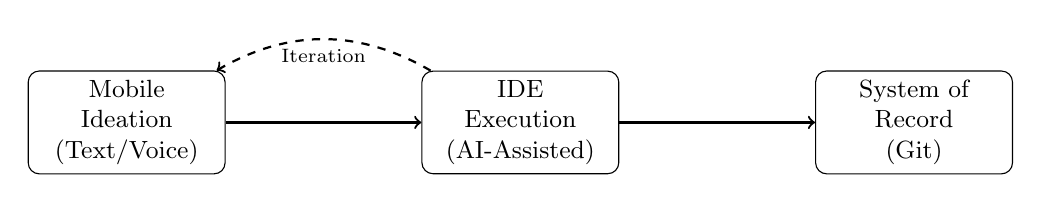
\begin{tikzpicture}[
    box/.style={rectangle, draw, rounded corners, minimum width=2.5cm, minimum height=1.2cm, align=center, font=\small},
    arrow/.style={->, thick}
]
\node[box] (mobile) at (0,0) {Mobile\\Ideation\\(Text/Voice)};
\node[box] (ide) at (5,0) {IDE\\Execution\\(AI-Assisted)};
\node[box] (git) at (10,0) {System of\\Record\\(Git)};

\draw[arrow] (mobile) -- (ide);
\draw[arrow] (ide) -- (git);
\draw[arrow, dashed] (ide) to[bend right=30] node[below, font=\scriptsize] {Iteration} (mobile);
\end{tikzpicture}
\end{center}

\vspace{1em}

\begin{columns}
\column{0.33\textwidth}
\textbf{Phase 1: Ideation}
\begin{itemize}
\scriptsize
\item Smartphone-based
\item Text/voice input
\item Problem framing
\end{itemize}

\column{0.33\textwidth}
\textbf{Phase 2: Execution}
\begin{itemize}
\scriptsize
\item Modern IDE
\item AI assistance
\item Trust boundary
\end{itemize}

\column{0.33\textwidth}
\textbf{Phase 3: Record}
\begin{itemize}
\scriptsize
\item Version control
\item History/rationale
\item Authoritative
\end{itemize}
\end{columns}
\end{frame}

\begin{frame}{Functional Requirements}
\begin{table}
\begin{tabular}{@{}lll@{}}
\toprule
\textbf{ID} & \textbf{Requirement} & \textbf{Type} \\
\midrule
FR-1 & Mobile ideation capability & Mandatory \\
FR-2 & IDE-centric execution with AI & Mandatory \\
FR-3 & Git-based system of record & Mandatory \\
FR-4 & Identity and trust boundary alignment & Mandatory \\
FR-5 & High-signal communication model & Recommended \\
\bottomrule
\end{tabular}
\end{table}
\end{frame}

\begin{frame}{Security and Compliance}
\begin{columns}
\column{0.5\textwidth}
\textbf{Trust Boundary Alignment}
\begin{itemize}
\item Security at authenticated identity
\item Security at managed device
\item AI operates in-boundary
\item No handling rules relaxed
\end{itemize}

\column{0.5\textwidth}
\textbf{Information Handling}
\begin{itemize}
\item No sensitive PII
\item No CUI
\item No proprietary information
\item No classified information
\end{itemize}
\end{columns}
\end{frame}

\begin{frame}{Value Proposition}
\begin{table}
\small
\begin{tabular}{@{}lll@{}}
\toprule
\textbf{Capability} & \textbf{Current} & \textbf{Proposed} \\
\midrule
Work capture & Fragmented, untracked & Structured, versioned \\
AI assistance & Outside boundary & In-boundary, modular \\
Knowledge preservation & At-risk & Durable artifacts \\
Automation readiness & Limited & Maximized \\
Auditability & Manual effort & Built-in traceability \\
\bottomrule
\end{tabular}
\end{table}
\end{frame}

\begin{frame}{Implementation Approach}
This demonstration is:

\vspace{1em}

\begin{itemize}
\item \textbf{Concrete enough to execute}
\begin{itemize}
\item Working repository
\item Defined outputs
\end{itemize}

\item \textbf{Abstract enough to remain vendor-neutral}
\begin{itemize}
\item Requirements-level specification
\item Implementation choices documented separately
\end{itemize}

\item \textbf{Self-demonstrating}
\begin{itemize}
\item Built using the proposed workflow
\end{itemize}
\end{itemize}
\end{frame}

\begin{frame}{Expected Outputs}
\begin{enumerate}
\item \textbf{Briefing Deck} --- This document (vendor-neutral)
\item \textbf{Repository Structure} --- Git-based with artifacts
\item \textbf{Verification Compliance Statement} --- Explicit evidence
\item \textbf{Traceability Matrix} --- Requirements to evidence
\end{enumerate}

\vspace{1em}

\begin{table}
\begin{tabular}{@{}ll@{}}
\toprule
\textbf{Method} & \textbf{Application} \\
\midrule
Inspection & Document review \\
Analysis & Compliance assessment \\
Demonstration & Working repository \\
\bottomrule
\end{tabular}
\end{table}
\end{frame}

\begin{frame}{Recommendation}
Adopt the SpeakUp workflow model as a pattern for:

\vspace{1em}

\begin{itemize}
\item Converting thinking into durable, reviewable artifacts
\item Preserving institutional knowledge
\item Enabling automation and auditability
\item Maintaining security and trust boundaries
\end{itemize}
\end{frame}

\begin{frame}{Next Steps}
\begin{enumerate}
\item Review this briefing
\item Identify pilot application area
\item Establish repository and workflow
\item Iterate between ideation and execution
\item Measure and refine
\end{enumerate}

\vspace{2em}

\begin{center}
\textit{This briefing was produced using the SpeakUp workflow model it describes.}
\end{center}
\end{frame}

\end{document}
